\documentclass[9pt,twocolumn,twoside,lineno]{pnas-new}
% Use the lineno option to display guide line numbers if required.

\templatetype{pnasresearcharticle} % Choose template 
% {pnasresearcharticle} = Template for a two-column research article
% {pnasmathematics} %= Template for a one-column mathematics article
% {pnasinvited} %= Template for a PNAS invited submission

\title{The human visual system preserves the hierarchy of 2-dimensional pattern regularity}

% Use letters for affiliations, numbers to show equal authorship (if applicable) and to indicate the corresponding author
\author[a, b, 1]{Peter J. Kohler}
\author[c]{Alasdair D. F. Clarke}

\affil[a]{York University, Department of Psychology, Toronto, ON M3J 1P3, Canada}
\affil[b]{Centre for Vision Research, York University, Toronto, ON, M3J 1P3, Canada}
\affil[c]{Stanford University, Department of Psychology, Stanford, CA 94305, United States}
\affil[d]{University of Essex, Department of Psychology, Colchester, UK, CO4 3SQ}

% Please give the surname of the lead author for the running footer
\leadauthor{Kohler} 

% Please add here a significance statement to explain the relevance of your work
\significancestatement{Wallpaper groups were discovered in the mid-19th century, and the 17 groups constitute the complete set of possible ways of regularly tiling the 2D-plane. In recent years wallpaper groups have found use in the vision science community, as an ideal stimulus set for studying the perception of symmetries in textures. Here we present brain imaging and psychophysical data on the complete set of wallpaper groups and show the hierarchical organization among wallpaper groups in reflected in both representations in visual cortex and performance on a symmetry detection task. This shows that the visual system is highly sensitive to reguarities in textures, and suggest that symmetries may play an important role in texture perception.}

% Please include corresponding author, author contribution and author declaration information
\authorcontributions{PJK and ADFC designed the study, PJK collected EEG data, ADFC collected psychophysical data, PJK and ADFC wrote the paper.}
\authordeclaration{The authors have no conflicts of interests to declare}
\correspondingauthor{\textsuperscript{1}To whom correspondence should be addressed. E-mail: \href{mailto:pjkohler@syorku.ca}{pjkohler@yorku.ca}}

% Keywords are not mandatory, but authors are strongly encouraged to provide them. If provided, please include two to five keywords, separated by the pipe symbol, e.g:
\keywords{Keyword 1 $|$ Keyword 2 $|$ Keyword 3 $|$ ...} 

\begin{abstract}
A century of vision research has demonstrated that symmetry contributes to numerous domains of visual perception \cite{RN1311, RN1166,RN1682,RN1824}. In a 2-D image, the four fundamental symmetries, reflection, rotation, translation and glide reflection, can be combined in 17 distinct ways. These 17 “wallpaper” groups \cite{RN1562,RN1563,RN1425} obey a hierarchy, determined by mathematical group theory, in which simpler groups are subgroups of more complex ones\cite{RN1711}. Here we probe representations of symmetries in wallpaper groups using two methods: (1) Steady-State Visual Evoked Potentials (SSVEPs) recorded using EEG and (2) symmetry detection thresholds measured psychophysically. We find that hierarchical relationships between the wallpaper groups are almost perfectly preserved in both behavior and response amplitudes in visual cortex. This remarkable consistency between the structure of symmetry representations and mathematical group theory, is likely generated over visual development, through implicit learning of regularities in the environment. 
\end{abstract}

\dates{This manuscript was compiled on \today}
\doi{\url{www.pnas.org/cgi/doi/10.1073/pnas.XXXXXXXXXX}}

\begin{document}

\maketitle
\thispagestyle{firststyle}
\ifthenelse{\boolean{shortarticle}}{\ifthenelse{\boolean{singlecolumn}}{\abscontentformatted}{\abscontent}}{}

% If your first paragraph (i.e. with the \dropcap) contains a list environment (quote, quotation, theorem, definition, enumerate, itemize...), the line after the list may have some extra indentation. If this is the case, add \parshape=0 to the end of the list environment.
\dropcap{S}ymmetries are present at many scales in images of natural scenes, due to a complex interplay of physical forces that govern pattern formation in nature. The importance of symmetry for visual perception has been known at least since the gestalt movement of the early 20th century. Since then, symmetry has been shown to contribute to the perception of shapes \cite{RN1311,RN1682}, scenes \cite{RN1824} and surface properties \cite{RN1166}, as well as the social process of mate selection \cite{RN1337}. Most of this work has focused on mirror symmetry or \textit{reflection}, with much less attention being paid to the other fundamental symmetries: \textit{rotation}, \textit{translation} and \textit{glide reflection}. In the two spatial dimensions relevant for images, these four fundamental symmetries can be combined in 17 distinct ways, the “wallpaper” groups \cite{RN1562,RN1563,RN1425}. Previous work has focused on four of the wallpaper groups, and used functional MRI to show that rotation symmetries within wallpapers are represented parametrically in several areas in occipital cortex, beginning with visual area V3 \cite{RN1725}. This effect is also robust in electroencephalography (EEG), whether measured using Steady-State Visual Evoked Potentials (SSVEPs)\cite{RN1725} or event-related paradigms \cite{RN1959}. Here we extend on this work by collecting SSVEPs and psychophysical data from human participants viewing the complete set of wallpaper groups. We measure responses in visual cortex to 16 out of the 17 wallpaper groups, with the 17th serving as a control stimulus, with the goal of providing a more complete picture of how wallpaper groups are represented in the human visual system.

A wallpaper group is a topologically discrete group of isometries of the Euclidean plane, i.e. transformations that preserve distance \cite{RN1425}. Wallpaper groups differ in the number and kind of these transformations. In mathematical group theory, when the elements of one group is completely contained in another, the inner group is called a subgroup of the outer group \cite{RN1425}. Subgroup relationships between wallpaper groups can be distinguished by their indices. The index of a subgroup relationship is the number of cosets, i.e. the number of times the subgroup is found in the outer group \cite{RN1425}. As an example, let us consider groups P6 and P2. If we ignore the translations in two directions that both groups share, group P6 consists of the set of rotations {$0^{\circ}$, $60^{\circ}$, $120^{\circ}$, $180^{\circ}$, $240^{\circ}$, $300^{\circ}$}, in which P2 {$0^{\circ}$, $180^{\circ}$} is contained. P2 is thus a subgroup of P6, and the full P6 set can be generated by every combination of P2 and rotations {$0^{\circ}$, $120^{\circ}$, $240^{\circ}$}. Because P2 is repeated three times in P6, P2 is a subgroup of P6 with index 3 \cite{RN1425}. The 17 wallpaper groups thus obey a hierarchy of complexity where simpler groups are sub-groups of more complex ones \cite{RN1711}.

\begin{figure}[tb]
\centering
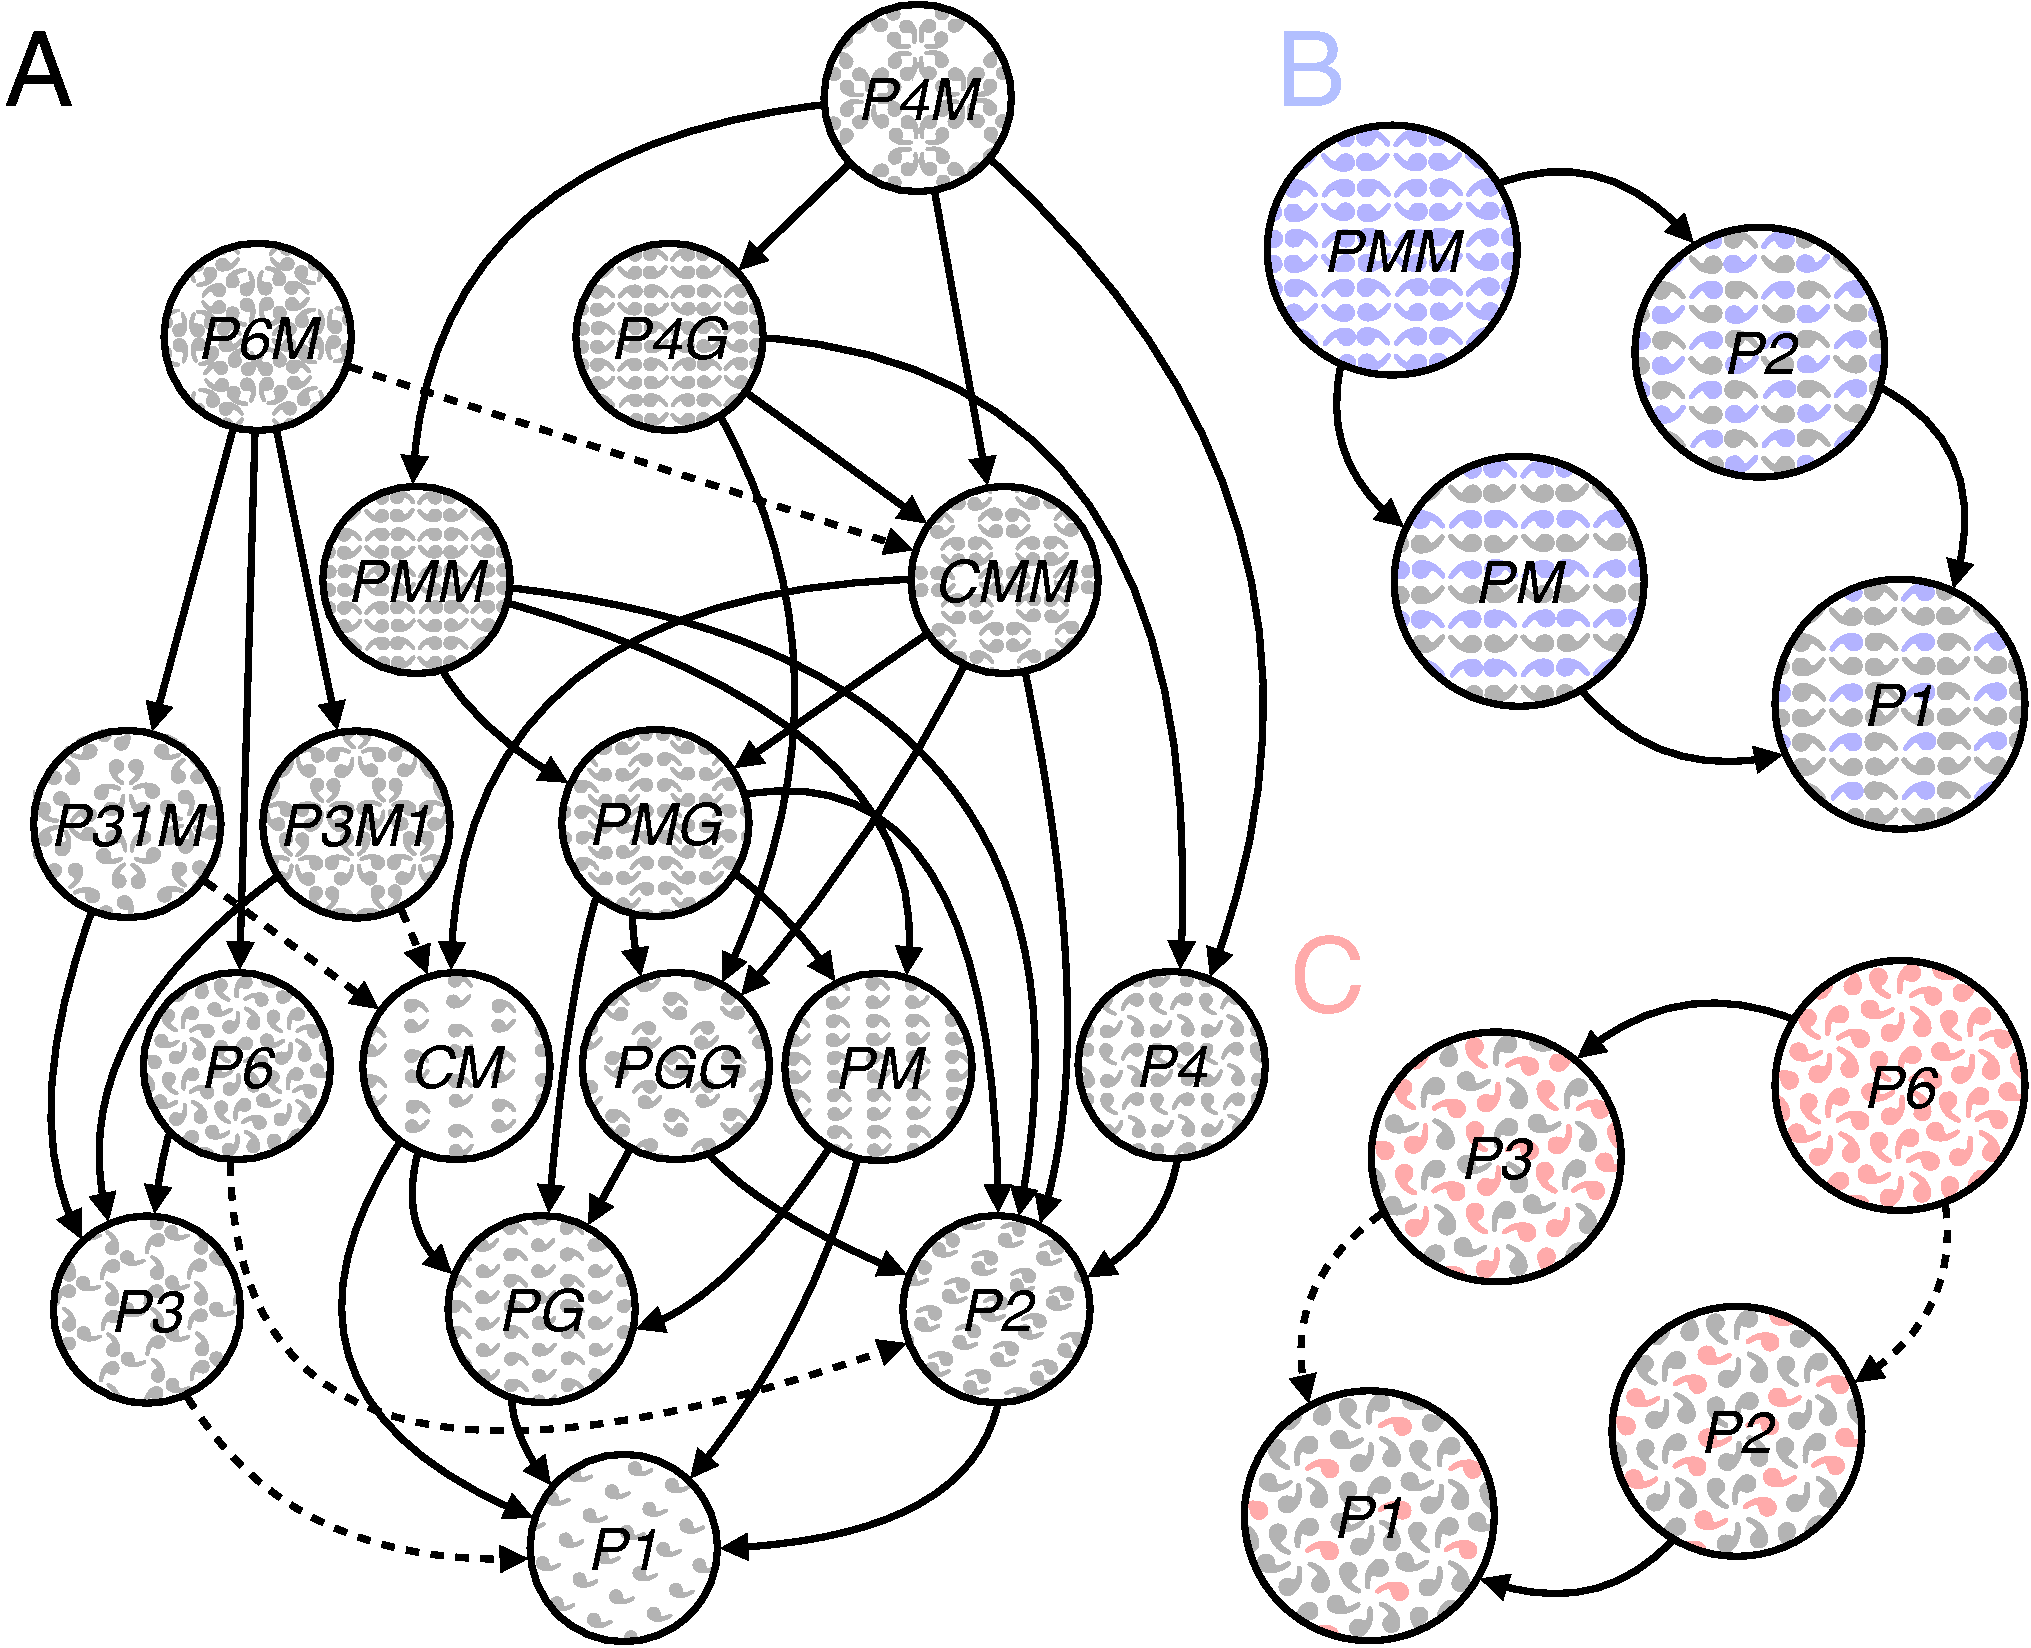
\includegraphics[width=1\linewidth]{../figures/figure1.png}
\caption{Examplar stimulus for each of the 16 wallpaper groups, with corresponding <something EEG> and a boxplot showing the distribution of display duration thresholds. }
\label{fig:durations_rotations}
\end{figure}

The two datasets presented here puts on in the position of being able to assess the extent to which both behavior and brain responses follow that hierachy. The results show that activity in human visual cortex is remarkably consistent with the hierarchical relationships between the wallpaper groups, with SSVEP amplitudes and psychophysical thresholds preserving these relationships at a level that is far beyond chance. Visual cortex thus appears to encode all of the fundamental symmetries using a representational structure that closely approximates the subgroup relationships from group theory. Given that most participants had no knowledge of group theory, the ordered structure of visual responses to wallpaper groups is likely learned implicitly from regularities in the visual environment.

\section*{Results}

The stimuli used in our two experiments were multiple exemplar images belonging to each of the wallpaper groups, generated from random-noise textures, as described in detail elsewhere \cite{RN1725}. Exemplar images from group P1 was used as control stimuli, and each exemplar from the other 16 groups had a power-spectrum matched P1 exemplar. The matched P1 exemplars were generated by phase-scrambling the exemplar images. Because all wallpapers are periodic due to their lattice tiling structure, the phase-scrambled images all belong to group P1 regardless of group membership of the original exemplar. P1 contains no symmetries other than translation, while all other groups contain translation in combination with one or more of the other three fundamental symmetries (reflection, rotation, glide reflection) \cite{RN1425}. In our SSVEP experiment, this stimulus set allowed us to isolate brain activity specific to the symmetry structure in the exemplar images from activity associated with modulation of low-level features, by alternating exemplar images and control exemplars. In this design, responses to structural features beyond the shared power spectrum, including any symmetries other than translation, are isolated in the odd harmonics of the image update frequency \cite{RN1725,RN1540, RN1954}. Thus, the combined magnitude of the odd harmonic response components can be used as a measure of the overall strength of the visual cortex response.

The psychophysical experiment took a distinct but related approach. In each trial an exemplar image was shown with its matched control, one image after the other, and the order varied pseudo-randomly such that in half the trials the original exemplar was shown first, and in the other half the control image was shown first. After each trial, participants were told to indicate whether the first or second image contained more structure, and the duration of both images was controlled by a staircase procedure so that a threshold duration could be computed for each wallpaper group. 

A summary of our results can be seen in Figure 1 ...



\begin{figure}%[tbhp]
\centering
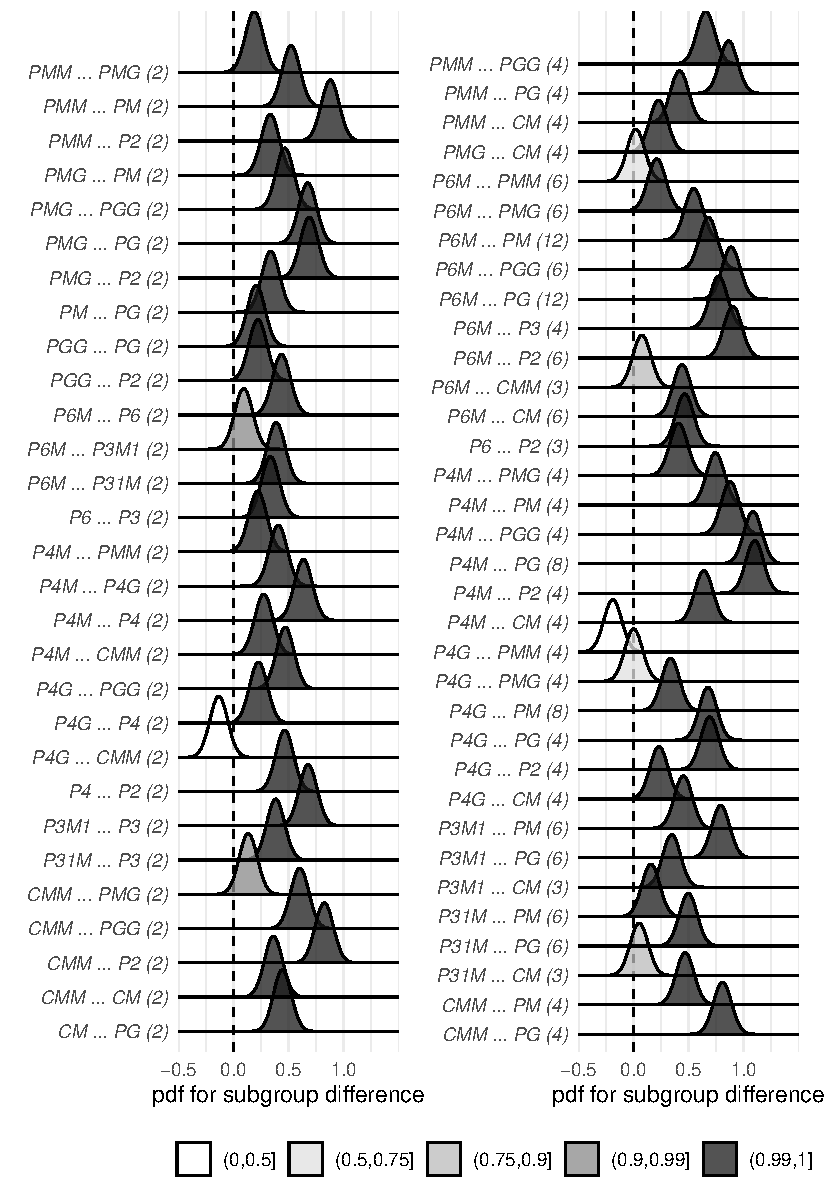
\includegraphics[width=1\linewidth]{../analysis/plots/subgroup_comp_eeg_rms.pdf}
\caption{Posterior distributions for the difference in mean RMS EEG response. Colour coding of the text indicates the index of the subgroup, while the colour of the filled distribution relates to the conditional probability that the difference in means is greater than zero. We can see that 55/64 subgroup relationships have $p(\Delta|data)>0.9$.}
\label{fig:durations_rotations}
\end{figure}

\begin{figure}%[tbhp]
\centering
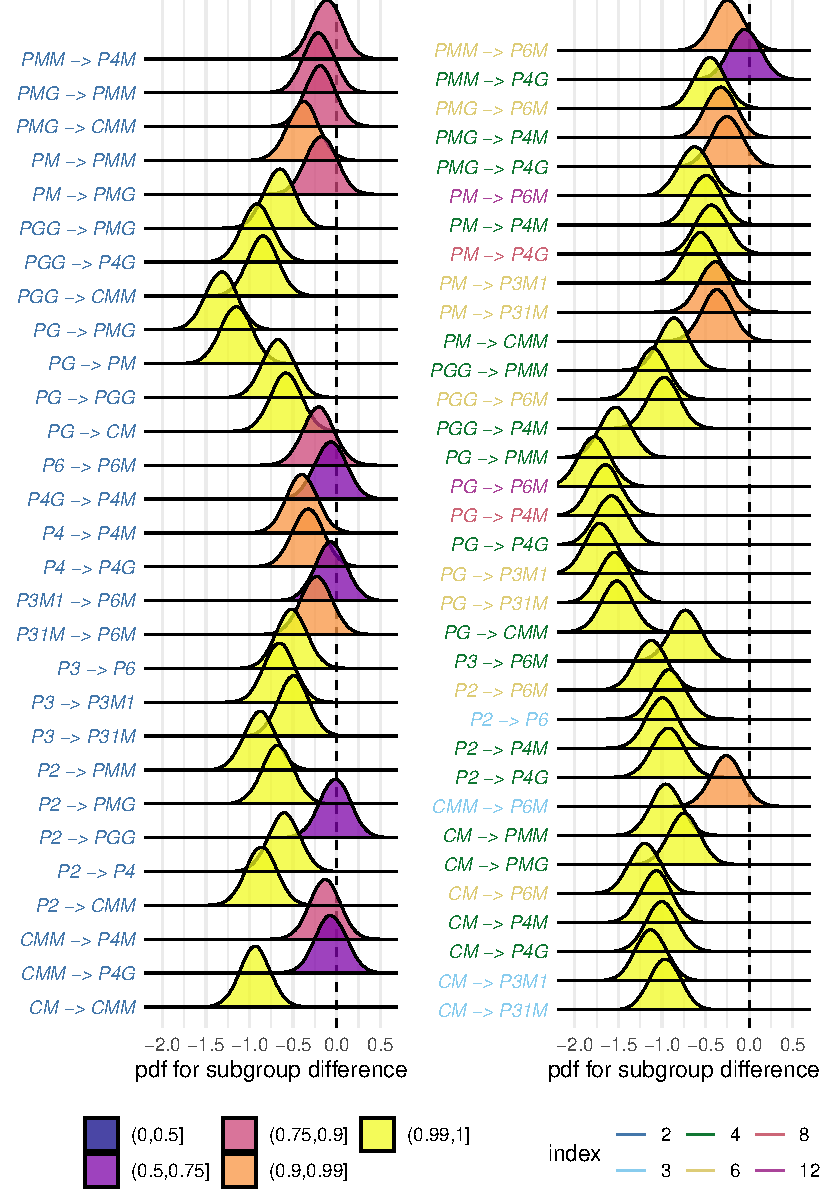
\includegraphics[width=1\linewidth]{../analysis/plots/subgroup_comp_psychophysical.pdf}
\caption{Posterior distributions for the difference in mean display duration threshold. Colour coding of the text indicates the index of the subgroup, while the colour of the filled distribution relates to the conditional probability that the difference in means is greater than zero. We can see that 55/64 subgroup relationships have $p(\Delta|data)>0.9$.}
\label{fig:durations_rotations}
\end{figure}

\begin{figure}%[tbhp]
\centering
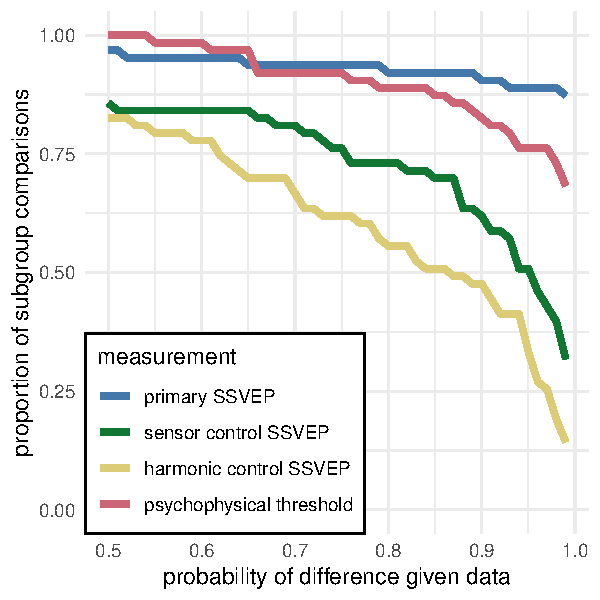
\includegraphics[width=1\linewidth]{../analysis/plots/model_roc_style.pdf}
\caption{Posterior distributions for the difference in mean RMS EEG response. Colour coding of the text indicates the index of the subgroup, while the colour of the filled distribution relates to the conditional probability that the difference in means is greater than zero. We can see that 55/64 subgroup relationships have $p(\Delta|data)>0.9$.}
\label{fig:durations_rotations}
\end{figure}


\section*{Discussion}

Here we show that beyond merely responding to the elementary symmetry operations of reflection \cite{RN1170} and rotation \cite{RN1725}, the visual system explicitly represents hierarchical structure of the 17 wallpaper groups, and thus the compositions of all four of the fundamental symmetry transformations (rotation, reflection, translation, glide reflection) which comprise regular textures. The RMS measure of SSVEP amplitude, preserves the complex hierarchy of subgroup relationships among the wallpaper groups \cite{RN1711}. Out of a total of 60 relationships, 53 were preserved in a significant number of participants, and 49 were significant even at a stricter threshold (p < 0.002). The ordering was highly stable in individual participants, with an average preservation rate of ~21 of 25 participants across all 60 relationships (see Figure 3). This remarkable consistency was specific to the odd harmonics of the stimulus frequency, that capture the symmetry-specific response \cite{RN1725} and to electrodes in an ROI over occipital cortex. When the same analysis was done on the even harmonics of the occipital cortex ROI, the ordering of responses was much less apparent (see Figure S2) and preservation rates much lower (see Figure S4). The odd harmonics from electrodes in an ROI over parietal cortex, showed even weaker evidence of preserving the hierarchy among sub-groups (see Figure S5). Importantly, no relationships were preserved in either of these control analyses that were not also preserved in the main analysis of the odd harmonics in the occipital cortex ROI. The current data provide a complete description of the visual system’s response to symmetries in the 2-D plane. Our design does not allow us to independently measure the response to P1, but because each of the 16 other groups produce non-zero odd harmonic amplitudes (see Figure 2), we can conclude that the relationships between P1 and all other groups, where P1 is the subgroup, are also preserved by the visual system. The subgroup relationships are not obvious perceptually, and most participants had no knowledge of group theory. Thus, the visual system’s ability to preserve the subgroup hierarchy does not depend on explicit knowledge of the relationships. Furthermore, behavioral experiments have shown that although naïve observers can distinguish many of the wallpaper groups \cite{RN1253}, they are generally error-prone when asked to assign exemplar images to the appropriate group \cite{RN172}. The correspondence between responses in the visual system and group theory that we demonstrate here, may reflect a form of implicit learning that depends on the structure of the natural world. The environment is itself constrained by physical forces underlying pattern formation and these forces are subject to multiple symmetry constraints \cite{RN1634}. The ordered structure of responses to wallpaper groups could be driven by a central tenet of neural coding, that of efficiency. If coding is to be efficient, neural resources should be distributed in such a way that the structure of the environment is captured with minimum redundancy considering the visual geometric optics, the capabilities of the subsequent neural coding stages and the behavioral goals of the organism \cite{RN1758, RN1760, RN1757, RN1756}. Early work within the efficient coding framework suggested that natural images had a $1/f$ spectrum and that the corresponding redundancy between pixels in natural images could be coded efficiently with a sparse set of oriented filter responses, such as those present in the early visual pathway \cite{RN1740, RN1446}. Our results suggest that the principle of efficient coding extends to a much higher level of structural redundancy – that of symmetries in visual images. The 17 wallpaper groups are completely regular, and relatively rare in the visual environment, especially when considering distortions due to perspective and occlusion. Near-regular textures, however abound in the visual world, and can be approximated as deformed versions of the wallpaper groups \cite{RN1519}. The correspondence between brain data and group theory demonstrated here may indicate that the visual system represents visual textures using a similar scheme, with the wallpaper groups serving as anchor points in representational space. This framework resembles norm-based encoding strategies that have been proposed for other stimulus classes, most notably faces \cite{RN435}, and leads to the prediction that adaptation to wallpaper patterns should distort perception of near-regular textures, similar to the aftereffects found for faces \cite{RN1768}. Field biologist have demonstrated that animals respond more strongly to exaggerated versions of a learned stimulus, referred to as “supernormal” stimuli \cite{RN1775}. In the norm-based encoding framework, wallpaper groups can be considered super-textures, exaggerated examples of the near-regular textures that surround us. Artists may consciously or unconsciously create supernormal stimuli, to capture the essence of the subject and evoke strong responses in the audience \cite{RN1764}. Wallpaper groups are visually compelling and have been widely used in human artistic expression going back to the Neolithic age \cite{RN1949}. If wallpapers are super-textures, their prevalence may be a direct consequence of the strategy the human visual system uses for encoding visual textures. 

\section*{snippets}
Specifically, the amplitudes of symmetry-specific responses in individual participants ($n=25$) preserve these relationships at an above-chance level in 88.3\% (53 out of 60) of cases.

we used a steady-state design, in which exemplar images belonging to 16 of the 17 wallpaper groups alternated with phase-scrambled images of the same group. 
Exemplars from each of the 16 groups alternated at 0.83 Hz with their corresponding set of P1 exemplars, that were matched in terms of their Fourier power spectrum. 

Thus, the magnitude of the odd harmonic response components can be used as a distance metric for each group, with distance being measured relative to the simplest group, P1. 

% \section*{Guide to using this template on Overleaf}

% Please note that whilst this template provides a preview of the typeset manuscript for submission, to help in this preparation, it will not necessarily be the final publication layout. For more detailed information please see the \href{http://www.pnas.org/site/authors/format.xhtml}{PNAS Information for Authors}.

% If you have a question while using this template on Overleaf, please use the help menu (``?'') on the top bar to search for \href{https://www.overleaf.com/help}{help and tutorials}. You can also \href{https://www.overleaf.com/contact}{contact the Overleaf support team} at any time with specific questions about your manuscript or feedback on the template.

% \subsection*{Author Affiliations}

% Include department, institution, and complete address, with the ZIP/postal code, for each author. Use lower case letters to match authors with institutions, as shown in the example. Authors with an ORCID ID may supply this information at submission.

% \subsection*{Submitting Manuscripts}

% All authors must submit their articles at \href{http://www.pnascentral.org/cgi-bin/main.plex}{PNAScentral}. If you are using Overleaf to write your article, you can use the ``Submit to PNAS'' option in the top bar of the editor window. 

% \subsection*{Format}

% Many authors find it useful to organize their manuscripts with the following order of sections;  Title, Author Affiliation, Keywords, Abstract, Significance Statement, Results, Discussion, Materials and methods, Acknowledgments, and References. Other orders and headings are permitted.

% \subsection*{Manuscript Length}

% PNAS generally uses a two-column format averaging 67 characters, including spaces, per line. The maximum length of a Direct Submission research article is six pages and a Direct Submission Plus research article is ten pages including all text, spaces, and the number of characters displaced by figures, tables, and equations.  When submitting tables, figures, and/or equations in addition to text, keep the text for your manuscript under 39,000 characters (including spaces) for Direct Submissions and 72,000 characters (including spaces) for Direct Submission Plus.

% \subsection*{Data Archival}

% PNAS must be able to archive the data essential to a published article. Where such archiving is not possible, deposition of data in public databases, such as GenBank, ArrayExpress, Protein Data Bank, Unidata, and others outlined in the Information for Authors, is acceptable.

% % \begin{SCfigure*}[\sidecaptionrelwidth][t]
% % \centering
% % % \includegraphics[width=11.4cm,height=11.4cm]{frog}
% % \caption{This caption would be placed at the side of the figure, rather than below it.}\label{fig:side}
% % \end{SCfigure*}

% \subsection*{Digital Figures}

% Only TIFF, EPS, and high-resolution PDF for Mac or PC are allowed for figures that will appear in the main text, and images must be final size. Authors may submit U3D or PRC files for 3D images; these must be accompanied by 2D representations in TIFF, EPS, or high-resolution PDF format.  Color images must be in RGB (red, green, blue) mode. Include the font files for any text. 

% Figures and Tables should be labelled and referenced in the standard way using the \verb|\label{}| and \verb|\ref{}| commands.

% Figure \ref{fig:frog} shows an example of how to insert a column-wide figure. To insert a figure wider than one column, please use the \verb|\begin{figure*}...\end{figure*}| environment. Figures wider than one column should be sized to 11.4 cm or 17.8 cm wide. Use \verb|\begin{SCfigure*}...\end{SCfigure*}| for a wide figure with side captions.

% \subsection*{Tables}
% In addition to including your tables within this manuscript file, PNAS requires that each table be uploaded to the submission separately as a “Table” file.  Please ensure that each table .tex file contains a preamble, the \verb|\begin{document}| command, and the \verb|\end{document}| command. This is necessary so that the submission system can convert each file to PDF.

% \subsection*{Single column equations}

% Authors may use 1- or 2-column equations in their article, according to their preference.

% To allow an equation to span both columns, use the \verb|\begin{figure*}...\end{figure*}| environment mentioned above for figures.

% Note that the use of the \verb|widetext| environment for equations is not recommended, and should not be used. 

% \begin{figure*}[bt!]
% \begin{align*}
% (x+y)^3&=(x+y)(x+y)^2\\
%        &=(x+y)(x^2+2xy+y^2) \numberthis \label{eqn:example} \\
%        &=x^3+3x^2y+3xy^3+x^3. 
% \end{align*}
% \end{figure*}


% \begin{table}%[tbhp]
% \centering
% \caption{Comparison of the fitted potential energy surfaces and ab initio benchmark electronic energy calculations}
% \begin{tabular}{lrrr}
% Species & CBS & CV & G3 \\
% \midrule
% 1. Acetaldehyde & 0.0 & 0.0 & 0.0 \\
% 2. Vinyl alcohol & 9.1 & 9.6 & 13.5 \\
% 3. Hydroxyethylidene & 50.8 & 51.2 & 54.0\\
% \bottomrule
% \end{tabular}

% \addtabletext{nomenclature for the TSs refers to the numbered species in the table.}
% \end{table}

% \subsection*{Supporting Information (SI)}

% Authors should submit SI as a single separate PDF file, combining all text, figures, tables, movie legends, and SI references.  PNAS will publish SI uncomposed, as the authors have provided it.  Additional details can be found here: \href{http://www.pnas.org/page/authors/journal-policies}{policy on SI}.  For SI formatting instructions click \href{https://www.pnascentral.org/cgi-bin/main.plex?form_type=display_auth_si_instructions}{here}.  The PNAS Overleaf SI template can be found \href{https://www.overleaf.com/latex/templates/pnas-template-for-supplementary-information/wqfsfqwyjtsd}{here}.  Refer to the SI Appendix in the manuscript at an appropriate point in the text. Number supporting figures and tables starting with S1, S2, etc.

% Authors who place detailed materials and methods in an SI Appendix must provide sufficient detail in the main text methods to enable a reader to follow the logic of the procedures and results and also must reference the SI methods. If a paper is fundamentally a study of a new method or technique, then the methods must be described completely in the main text.

% \subsubsection*{SI Datasets} 

% Supply Excel (.xls), RTF, or PDF files. This file type will be published in raw format and will not be edited or composed.

% \matmethods{Please describe your materials and methods here. This can be more than one paragraph, and may contain subsections and equations as required. Authors should include a statement in the methods section describing how readers will be able to access the data in the paper. 

\subsection*{Participants}
Twenty-five participants (11 females, mean age 28.7±13.3) took part in the EEG experiment. Their informed consent was obtained before the experiment under a protocol that was approved by the Institutional Review Board of Stanford University. 11 participants (8 females, mean age 20.73±1.21) took part in the psychophysics experiment. All participants had normal or corrected-to-normal vision. Their informed consent was obtained before the experiment under a protocol that was approved by the University of Essex's Ethics Committee.

\subsection*{Stimulus Generation}
Exemplars from the different wallpaper groups were generated using a modified version of the methodology developed by Clarke and colleagues\cite{RN172} that we have described in detail elsewhere\cite{RN1725}. Briefly, exemplar patterns for each group were generated from random-noise textures, which were then repeated and transformed to cover the plane, according to the symmetry axes and geometric lattice specific to each group. The use of noise textures as the starting point for stimulus generation allowed the creation of an almost infinite number of distinct exemplars of each wallpaper group. For each exemplar image, phase-randomized control exemplars were generated that had the same power spectrum as the exemplar images for each group. The phase scrambling eliminates rotation, reflection and glide-reflection symmetries within each exemplar, but the phase-scrambled images inherent the spectral periodicity arising from the periodic tiling. This means that all control exemplars, regardless of which wallpaper group they are derived from, degenerate to another symmetry group, namely P1. P1 is the simplest of the wallpaper groups, and contains only translations of a region whose shape derives from the lattice. Because the different wallpaper groups have different lattices, P1 controls matched to different groups have different power spectra. Our experimental design takes these differences into account by comparing the neural responses evoked by each wallpaper group to responses evoked by the matched control exemplars.

\subsection*{Stimulus Presentation}
Stimulus Presentation. For the EEG experiment, the stimuli were shown on a 24.5" Sony Trimaster EL PVM-2541 organic light emitting diode (OLED) display at a screen resolution of $1920\times1080$ pixels, 8-bit color depth and a refresh rate of 60 Hz, viewed at a distance of 70 cm. The mean luminance was 69.93 cd/m2 and contrast was 95\%. The diameter of the circular aperture in which the wallpaper pattern appeared was $13.8^\circ$ of visual angle presented against a mean luminance gray background. Stimulus presentation was controlled using in-house software.

For the psychophysics experiment, the stimuli were shown on a $48 \times 27$cm VIEWPixx/3D LCD Display monitor, model VPX-VPX-2005C, resolution $1920 \times 1080$ pixels, with a viewing distance of approximately 40cm and linear gamma. Stimulus presentation was controlled using MatLab and Psychtoolbox-3 \cite{kleiner2007,brainard1997spatial}. The diameter of the circular aperture for the stimuli was $21.5^\circ$.

\subsection*{EEG Procedure}
Visual Evoked Potentials were measured using a steady-state design, in which P1 control images alternated with test images from each of the 16 other wallpaper groups[2]. Exemplar images were always preceded by their matched P1 control image. A single 0.83 Hz stimulus cycle consisted of a control P1 image followed by an exemplar image, each shown for 600 ms. A trial consisted of 10 such cycles (12 sec) over which 10 different exemplar images and matched controls from the same rotation group were presented. For each group type, the individual exemplar images were always shown in the same order within the trials. Participants initiated each trial with a button-press, which allowed them to take breaks between trials. Trials from a single wallpaper group were presented in blocks of four repetitions, which were themselves repeated twice per session, and shown in random order within each session. To control fixation, the participants were instructed to fixate a small white cross in the center of display. To control vigilance, a contrast dimming task was employed. Two times per trial, an image pair was shown at reduced contrast, and the participants were instructed to press a button on a response pad. We adjusted the contrast reduction such that average accuracy for each participant was kept at ~85\% correct, so that the difficulty of the vigilance task was kept constant.     

\subsection*{Psychophysics Procedure}
The experiment consisted of 16 blocks, one for each of the wallpaper groups (excluding $P1$). In each trial, participants were presented with two stimuli (one of which was the wallpaper group for the current block of trials, the other being $P1$), one after the other (inter stimuli interval of 700ms). After each stimuli had been presented, it was masked with white noise for 300ms. After both stimuli had been presented, participants made a response on the keyboard to indicate whether they thought the first or second contained the most symmetry. Each block started with 10 practise trials, (stimulus display duration of 500ms) to allow participants to familiarise themselves with the current block's wallpaper pattern. If they achieved an accuracy of 9/10 in these trials they progressed to the rest of the block, otherwise they carried out another set of 10 practise trials. This process was repeated until the required accuracy of 9/10 was obtained. The rest of the block consisted of four interleaved staircases (using the QUEST algorithm \cite{watson1983quest}, full details given in the SI) of 30 trials each. On average, a block of trials took around 10 minutes to complete. 

\subsection*{EEG Acquisition and Preprocessing}
Electroencephalogram Acquisition and Preprocessing. The time-locked Steady-State Visual Evoked Potentials were collected with 128-sensor HydroCell Sensor Nets (Electrical Geodesics, Eugene, OR) and were band-pass filtered from 0.3 to 50 Hz. Raw data were evaluated off line according to a sample-by-sample thresholding procedure to remove noisy sensors that were replaced by the average of the six nearest spatial neighbors. On average, less than 5\% of the electrodes were substituted; these electrodes were mainly located near the forehead or the ears. The substitutions can be expected to have a negligible impact on our results, as the majority of our signal can be expected to come from electrodes over occipital, temporal and parietal cortices. After this operation, the waveforms were re-referenced to the common average of all the sensors. The data from each 12s trial were segmented into five 2.4 s long epochs (i.e., each of these epochs was exactly 2 cycles of image modulation). Epochs for which a large percentage of data samples exceeding a noise threshold (depending on the participant and ranging between 25 and 50 $\mu$V) were excluded from the analysis on a sensor-by-sensor basis. This was typically the case for epochs containing artifacts, such as blinks or eye movements. The use of steady-state stimulation drives cortical responses at specific frequencies directly tied to the stimulus frequency. It is thus appropriate to quantify these responses in terms of both phase and amplitude. Therefore, a Fourier analysis was applied on every remaining epoch using a discrete Fourier transform with a rectangular window. The use of epochs two-cycles (i.e., 2.4 s) long, was motivated by the need to have a relatively high resolution in the frequency domain, $\delta$f = 0.42 Hz. For each frequency bin, the complex-valued Fourier coefficients were then averaged across all epochs within each trial. Each participant did two sessions of 8 trials per condition, which resulted in a total of 16 trials per condition.

\subsection*{EEG Analysis}
Response waveforms were generated for each group by selective filtering in the frequency domain. For each participant, the average Fourier coefficients from the two sessions were averaged over trials and sessions. The Steady-State Visual Evoked Potentials paradigm we used allowed us to separate symmetry-related responses from non-specific contrast transient responses. Previous work has demonstrated that symmetry-related responses are predominantly found in the odd harmonics of the stimulus frequency, whereas the even harmonics consist mainly of responses unrelated to symmetry, that arise from the contrast change associated with the appearance of the second image[2-4]. This functional distinction of the harmonics allowed us to generate a single-cycle waveform containing the response specific to symmetry, by filtering out the even harmonics in the spectral domain, and then back-transforming the remaining signal, consisting only of odd harmonics, into the time-domain. For our main analysis, we averaged the odd harmonic single-cycle waveforms within a six-electrode region of interest (ROI) over occipital cortex (electrodes 70, 74, 75, 81, 82, 83). These waveforms, averaged over participants, are shown in Figure 2 in the main paper. The same analysis was done for the even harmonics (see Figure S1) and for the odd harmonics within a six electrode ROI over parietal cortex (electrodes 53, 54, 61, 78, 79, 86; see Figure S2). The root-mean square values of these waveforms, for each individual participant, were used to determine whether each of the wallpaper subgroup relationships were preserved in the brain data.  

\subsection*{Bayesian Analysis of EEG and Psychophysical data}
Bayesian analysis was carried out using R (v3.6.1) \cite{R} with the \texttt{brms} package (v2.9.0) \cite{burkner2017} and rStan (v2.19.2 \cite{rStan}). The data from each experiment were modelled using a Bayesian generalised mixed effect model with wallpaper group being treated as a 16 level factor, and random effects for participant. The EEG data and display thresholds were modelled using log-normal distributions with weakly informative, $ \mathcal{N}(0, 2)$, priors. After fitting the model to the data, samples were drawn from the posterior distribution for each mean of the EEG response (display duration) for each wallpaper group. These samples were then recombined to calculate the distribution of differences for each pair of subgroup and super-group. These distributions were then summarised by computing the conditional probability of obtaining a positive (negative) difference, $p(\Delta | data)$.

For further technical details, please see the supplementary materials where the full R code, model specification, prior and posterior predicitive checks, and model diagnoastics, can be found. 







\showmatmethods{} % Display the Materials and Methods section

\acknow{Please include your acknowledgments here, set in a single paragraph. Please do not include any acknowledgments in the Supporting Information, or anywhere else in the manuscript.}

\showacknow{} % Display the acknowledgments section

% Bibliography
\bibliographystyle{pnas-new} 
\bibliography{literature}

\end{document}